\chapter{Adders}
\label{ch:adders}

%%\textit{ripple-carry adders, twos complement, subtraction, \dots}

\section{Adding Numerals}
\label{sec:addition-by-numeral}

When people do paper-and-pencil arithmetic,
they use numerals.
For example, to add two numbers, a person
writes down the decimal numerals for the numbers,
one under the other with the digits lined up so that
the units digit of one number is directly under
the units digit of the other, and similarly for
the tens digits, hundreds digits, and so on.
Then, the units digits are added together,
and the low-order digit of that sum is written
in the units-digit column.

If the sum of the units digit is ten or more,
a "carry" is indicated in the tens-digit column.
The sum of the tens digits is computed and the
carry (if there was one) added to the sum.
As before, the low-order digit of the sum of the
tens digits (and carry) goes in the numeral for the sum,
but this time in tens-digit column.
A carry is marked, if necessary,
in the hundreds digit column.
This process moves across the digits of the addends until all the digits
are accounted for (Figure~\ref{fig:adding-decimal-numerals}).

\begin{figure}
\begin{center}
\begin{minipage}[b]{0.4\textwidth}
\begin{verbatim}
   11 1    carries
    ----
    9542   first addend
  +  638   second addend
    ----
   10180   sum
\end{verbatim}
\end{minipage}
\end{center}
\caption{Adding Decimal Numerals}
\label{fig:adding-decimal-numerals}
\end{figure}

To perform addition in this way, a person needs to know
the table for one-digit sums (0+0=0, 0+1=1, \dots 2+2=4 \dots 9+8=17, 9+9=18).
There are a hundred entries in the table ($10 \times 10$, one for each
possible pair of decimal digits).

Decimal numerals are not the only kind,
and addition can be carried out similarly, regardless of numeral base.
The table of one-digit sums is much smaller for binary numerals
than for decimal numerals because it only has to account for $0$ and $1$,
not $0$, $1$, $2$, \dots $9$, but
the process of adding numerals is in other respects
the same (Figure~\ref{fig:adding-binary-numerals}).
The small size of the one-digit-sum table simplifies the
both pencil-and-paper process and the difficulty of designing
digital circuits for performing addition on binary numerals, compared to what
it would be for decimal numerals.

\begin{figure}[!tbp]
\begin{center}
\begin{minipage}[b]{0.4\textwidth}
\begin{verbatim}
   11 111 1    carries
    --------
    01011101   first addend
  + 11010101   second addend
    --------
   100110010   sum
\end{verbatim}
\end{minipage}
\hfill
\begin{minipage}[b]{0.4\textwidth}
~~~~~~\emph{one-bit addition}\\
\vspace{.05 in}
\begin{tabular}{|c|c|c|c}
 \hline
 $+$      & $c$ & $s$ \\
 \hline
 $0+0$    & $0$ & $0$ \\
 \hline
 $0+1$    & $0$ & $1$ \\
% \hline
% $1+0$    & $0$ & $1$ \\
 \hline
 $1+1$    & $1$ & $0$ \\
 \hline
 $1+1+1$  & $1$ & $1$ \\
 \hline
\end{tabular}
\end{minipage}
\end{center}
\caption{Adding Binary Numerals}
\label{fig:adding-binary-numerals}
\end{figure}

\begin{ExerciseList}
\Exercise Describe by example the process of multiplying a pair of decimal numerals.

\Exercise Describe by example the process of multiplying a pair of binary numerals.
\end{ExerciseList}

\section{Adding One-Bit Binary Numerals}
\label{sec:adding-1-bit-numerals}

The addition table for one-bit, binary numerals
has only four entries, as shown in
Figure~\ref{fig:half-adder} (page \pageref{fig:half-adder}).
In the figure, the sum is shown in all four cases as two separate bits,
a carry bit $c$ and a sum bit $s$.
A close look at the table shows that
the carry bit matches the table of values of the
digital gate for logical-and (Figure \ref{fig-02-logic-gates}).
That is, the carry bit is 1 only if both inputs are 1s.
Otherwise, the carry bit is 0.
So, constructing a digital circuit to compute the carry bit
in the addition of two one-bit, binary numerals is simply
a matter of feeding the signals for the one-bit numerals
into a logical-and gate.

Another close look reveals that the sum bit
matches the table of values of the
digital gate for exclusive-or (Figure \ref{fig-02-logic-gates}).
That is, the sum bit is 0 if the two inputs are the same
and 1 if they are different.
So, constructing a digital circuit to compute the sum bit
amounts to feeding the signals for the one-bit numerals
into an exclusive-or gate.
Combining these ideas for carry-bit and sum-bit circuits
leads to a two-input, two-output circuit known as a
half-adder (Figure \ref{fig:half-adder}, page \pageref{fig:half-adder}).

\begin{figure}
\begin{center}
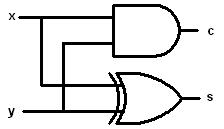
\includegraphics[scale=0.23]{Images/half-adder.png}
\todo{Improvised with PowerPoint. Redraw using Visio.}
\begin{Verbatim}
(defun and-gate (x y) (if (and (= x 1) (= y 1)) 1 0))
(defun or-gate (x y) (or (= x 1) (= y 1)))
(defun xor-gate (x y) (if (and (= x 1) (= y 1)) 0 (or-gate x y)))
(defun half-adder (x y) (list (xor-gate x y) (and-gate x y)))
\end{Verbatim}
\end{center}
\caption{Half-Adder Circuit and ACL2 Model}
\label{fig:half-adder}
\end{figure}

Since we reason about digital circuits using the methods
of Boolean algebra, we need an algebraic representation
of the circuit-diagram for the half-adder circuit.
Remember, digital circuits are only one of four
equivalent representations of Boolean formulas that
we have studied: circuit diagrams, well-formed formulas
in the notation of mathematical logic (for example, $x \wedge y$),
Boolean formulas in engineering notation (justaposition for $\wedge$,
$+$ for $\vee$, and over-bar for $\neg$), and ACL2 notation.
The ACL2 formalization allows us mechanize some aspects of the reasoning process.
So, Figure \ref{fig:half-adder} also specifies the half-adder circuit in ACL2 terms.
We refer to this specification as an
ACL2 model of the half-adder circuit.
It delivers the two output signals as a list of two elements,
the first element being the sum bit and the second, the carry bit.

In the end, we would like to have a circuit
that adds binary numerals,
and we saw in an example (Figure \ref{fig:adding-binary-numerals})
that this would require us to deal with three input bits
for each bit in the numerals:
the corresponding bits in the two addends
and the carry bit from the previous column.
The half-adder circuit is not up to this task,
since it has only two input signals.
However, we can put together a full-adder circuit
by combining two half-adders with an or-gate,
as shown in the circuit of Figure \ref{fig:full-adder}
(page \pageref{fig:full-adder}).
Since the full-adder circuit has three inputs,
each of which is either 0 or 1,
there are exactly eight possible input configurations,
as shown in the full-adder table.

\begin{figure}
\begin{center}
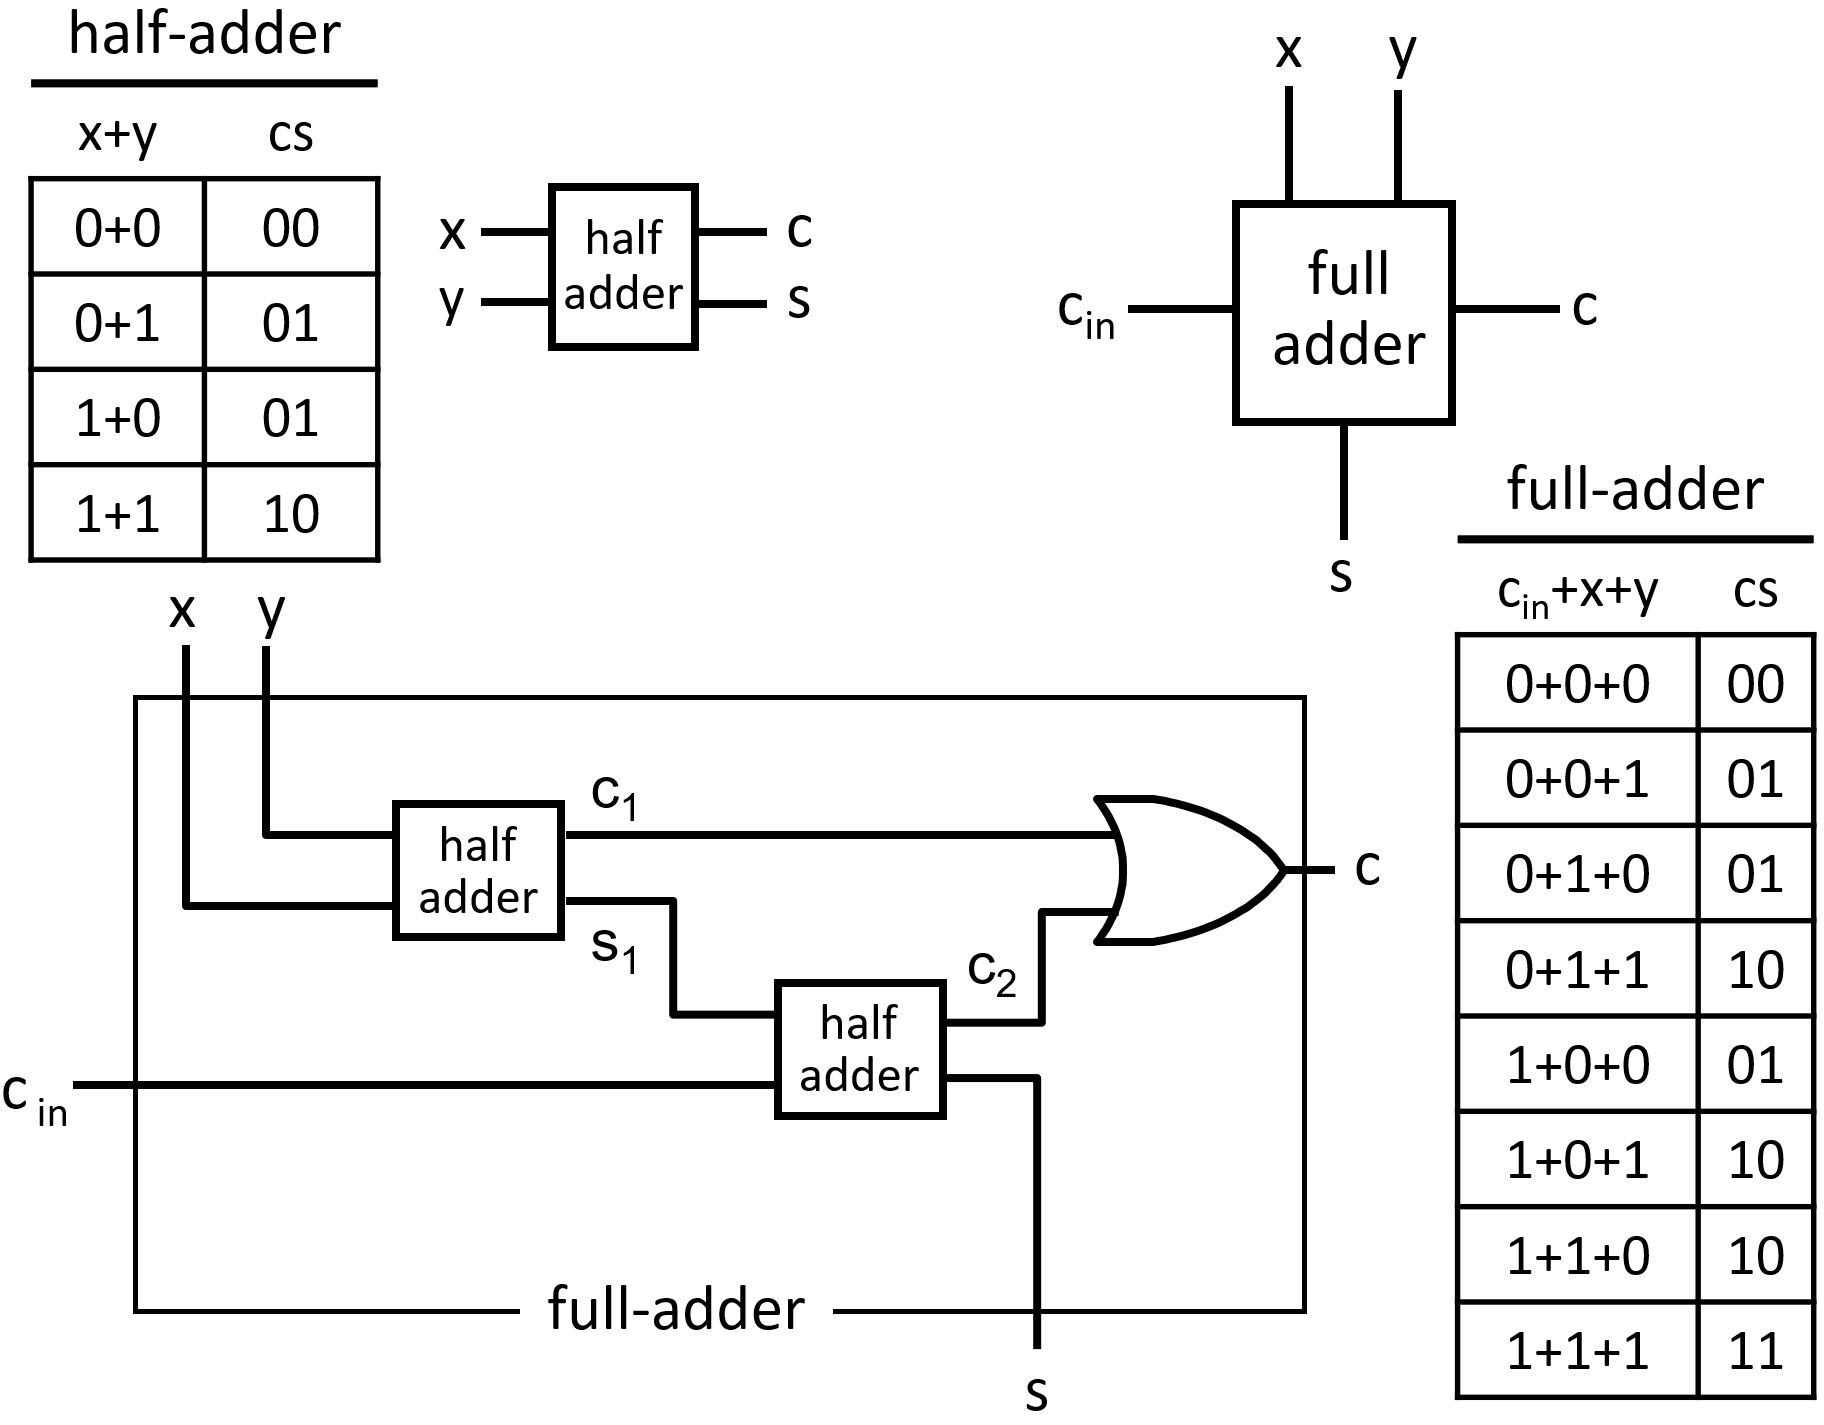
\includegraphics[scale=0.25]{Images/full-adder.png}
\todo{Improvised with PowerPoint. Redraw using Visio.}
\begin{Verbatim}
(defun full-adder (c-in x y)
  (let* ((h1 (half-adder x y))
         (s1 (first h1)) (c1 (second h1))
         (h2 (half-adder s1 c-in))
         (s  (first h2)) (c2 (second h2))
         (c  (or-gate c1 c2)))
    (list s c)))
\end{Verbatim}
\end{center}
\caption{Full-Adder Circuit and ACL2 Model}
\label{fig:full-adder}
\end{figure}

The full-adder operator defined in the figure
is a formal model in ACL2 of the circuit diagram,
and the following tests, one for each line in the table,
comprise a comprehensive, mechanized verification of
the model.
That makes it safe to use the full-adder as a component
in the design of a circuit to carry out addition on binary numerals
with more than one bit.

\label{full-adder-model-check}
\begin{Verbatim}
(check-expect (full-adder 0 0 0) (list 0 0))
(check-expect (full-adder 0 0 1) (list 1 0))
(check-expect (full-adder 0 1 0) (list 1 0))
(check-expect (full-adder 0 1 1) (list 0 1))
(check-expect (full-adder 1 0 0) (list 1 0))
(check-expect (full-adder 1 0 1) (list 0 1))
(check-expect (full-adder 1 1 0) (list 0 1))
(check-expect (full-adder 1 1 1) (list 1 1))
\end{Verbatim}

Instead of viewing the full-adder operands
as symbols for bits, we could use the numb operator
to interpret them as numbers.
If $x$ is a bit, then [$x$] is a numeral for
the number it denotes, and the \{\emph{Horner 2}\} theorem
(Exercise \ref{horner2-thm}, page \pageref{horner2-thm})
asserts that (numb [$x$]) computes that number.
The same theorem asserts that if $s$ and $c$ are bits,
then (numb [$s$ $c$]) is  the number that the numeral [$s$ $c$] denotes.
Combining these observations with the full-adder table
(Figure \ref{fig:full-adder}, page \pageref{fig:full-adder})
verifies the theorem \{full-adder ok\} shown in
Figure \ref{fig:full-adder-thm} (page \pageref{fig:full-adder-thm}),
both in paper-and-pencil form and in ACL2 notation.\footnote{The
full-adder operator delivers a list [$s$ $c$] whose first
element is the sum bit and whose second element is the carry bit.
The order of elements in the result delivered by full-adder was designed
to form a numeral for the sum of its three, one-bit operands.}

\begin{figure}
\begin{center}
\begin{tabular}{ll}
Theorem \{\emph{full-adder ok}\} & (numb [$s$ $c$]) $=$ (numb [$x$]) + (numb [$y$]) + (numb [$c_{in}$]) \\
                                 & where [$s$ $c$] = (full-adder $c_{in}$ $x$ $y$) \\
\end{tabular}
\begin{Verbatim}
(defthm full-adder-ok
  (= (numb (full-adder c-in x y))
     (+ (numb (list c-in)) (numb (list x)) (numb (list y)))))
\end{Verbatim}
\end{center}
\caption{Full-Adder Theorem}
\label{fig:full-adder-thm}
\end{figure}

\section{Adding Two-Bit Binary Numerals}
\label{sec:adding-2-bit-numerals}

Adding binary numerals with two bits is simply a matter
of connecting two full-adder circuits in a manner that
directs the output carry-bit produced by adding the low-order bits
to the input carry-bit of the second full-adder circuit.
Since there is never a carry into the low-order position,
we just supply zero as the carry-in for the full-adder circuit
that deals with the low-order bit.

\begin{figure}
\begin{center}
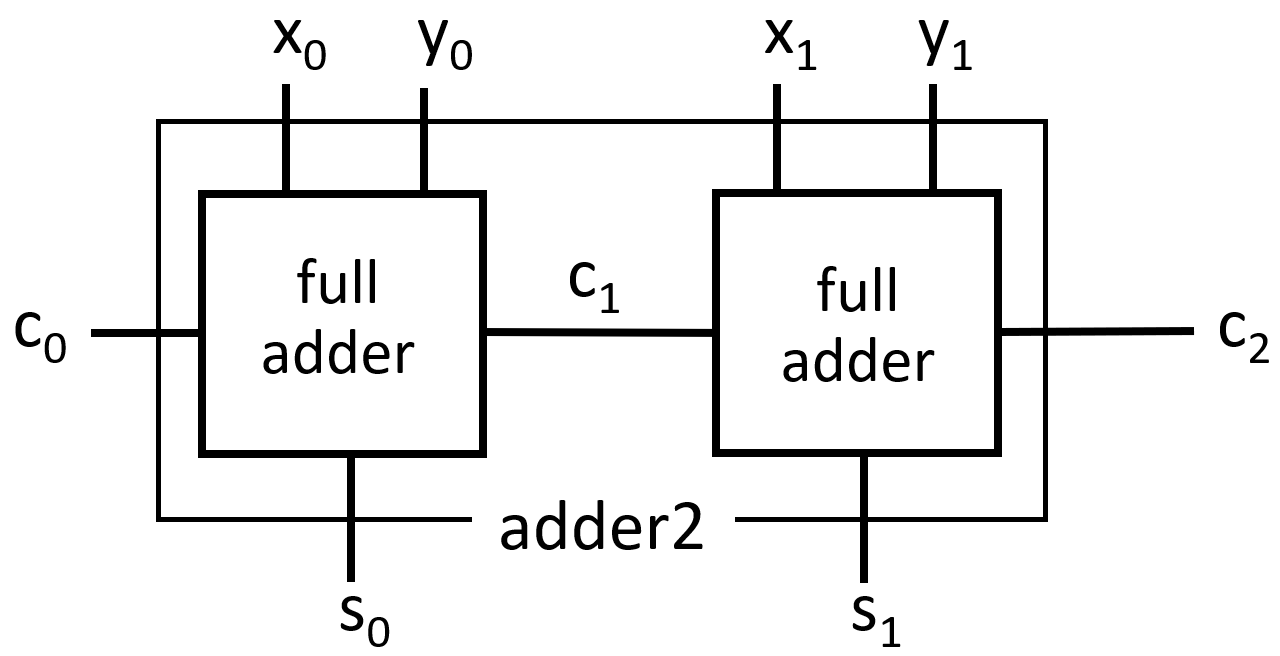
\includegraphics[scale=0.25]{Images/adder2.png}
\todo{Improvised with PowerPoint. Redraw using Visio.}
\begin{Verbatim}
(defun adder2 (c0 x y)
  (let* ((x0 (first x)) (x1 (second x))
         (y0 (first y)) (y1 (second y))
         (f0 (full-adder c0 x0 y0))
         (s0 (first f0)) (c1 (second f0))
         (f1 (full-adder c1 x1 y1))
         (s1 (first f1)) (c2 (second f1)))
    (list (list s0 s1) c2)))
\end{Verbatim}
\end{center}
\caption{Two-Bit Adder and ACL2 Model}
\label{fig:adder2}
\end{figure}

This two-bit addition circuit takes two, two-bit binary numerals
[$x_0$ $x_1$] and [$y_0$ $y_1$] as inputs, and
delivers as output a two-bit numeral along with a carry-bit,
as shown in Figure \ref{fig:adder2} (\pageref{fig:adder2}).
We refer to the output two-bit numeral, without the carry bit,
as the sum bits.
Ignoring the carry bit amounts to doing
modular arithmetic, mod 4 (that is, mod $2^2$).
This is confirmed by theorem \{\emph{pfx-mod}\} (page \pageref{pfx-mod}).

A mechanized verification of the arithmetic properties of adder2
could be constructed as a comprehensive test,
as we did with the full-adder for one-bit addition
(page \pageref{full-adder-model-check}).
However, there would be 32 cases to check
because there are five bits of input
(a carry-in and two bits in each numeral, $2^5$ combinations in all).
That makes a comprehensive test tedious to construct,
and it's easy to make a mistake.

A better approach is to think of a formula in logic that expresses
the properties we expect the model to have,
along the lines of the \{full-adder ok\} theorem
(Figure \ref{fig:full-adder-thm}, page \pageref{fig:full-adder-thm}).
To this end, we observe
that if we compute the sum of the three numbers represented by the two input
numerals and the input carry,
the total must add up to the number represented
by a numeral formed from the output sum-bits and
the output carry-bit.
The theorem is an equation between the
sum of the numeric interpretation of the input numerals
along with the input carry
and the numeric interpretation of the output numeral
together with the output carry.
As in the \{full-adder ok\} theorem,
the \{\emph{adder2-ok}\} theorem that specifies
the crucial, arithmetic property of the two-bit adder
uses the numb operator (page \pageref{nmb-defun})
to interpret binary numerals as numbers.

\begin{Verbatim}
(defthm adder2-ok
  (let* ((a (adder2 c0 (list x0 x1) (list y0 y1)))
         (s (first a)) (c (second a)))
    (= (numb (append s (list c)))
       (+ (numb(list c0))
          (numb (list x0 x1))
          (numb (list y0 y1))))))
\end{Verbatim}
\label{adder2-ok}

\begin{ExerciseList}
\Exercise Define a doublecheck property that tests
for correctness of the two-bit adder model
(Figure \ref{fig:adder2}, page \pageref{fig:adder2}).
Run the test using Proof Pad.
\emph{Note}: The data generator (random-between 0 1) delivers
a 0 or a 1 at random.

\Exercise By default, Proof Pad repeats the test fifty times
with random data
when it runs a doublecheck test.
How many random tests do you think would be needed to be reasonably
confident that all 32 different cases for the two-bit adder have been tested?
\end{ExerciseList}

\section{Adding w-Bit Binary Numerals}
\label{sec:adding-w-bit-numerals}

By now, you can predict what a circuit for adding three-bit
binary numerals would look like.
Just put another full adder in the circuit, and feed the
carry from adding the two low-order bits into the carry-in
of the new full-adder in the circuit, along with
the high-order bits in the two numerals.

Producing the circuit diagram for any number of bits
is just a matter of wiring the appropriate number of
full-adder components together in the appropriate way.
Figure \ref{fig:adder} (page \pageref{fig:adder}) presents a schematic 
for a circuit that adds \emph{w}-bit numerals.
The circuit is known as a ``ripple-carry adder'' because
of the way the carry-bit propagates across the line
of full-adder components.

\begin{figure}
\begin{center}
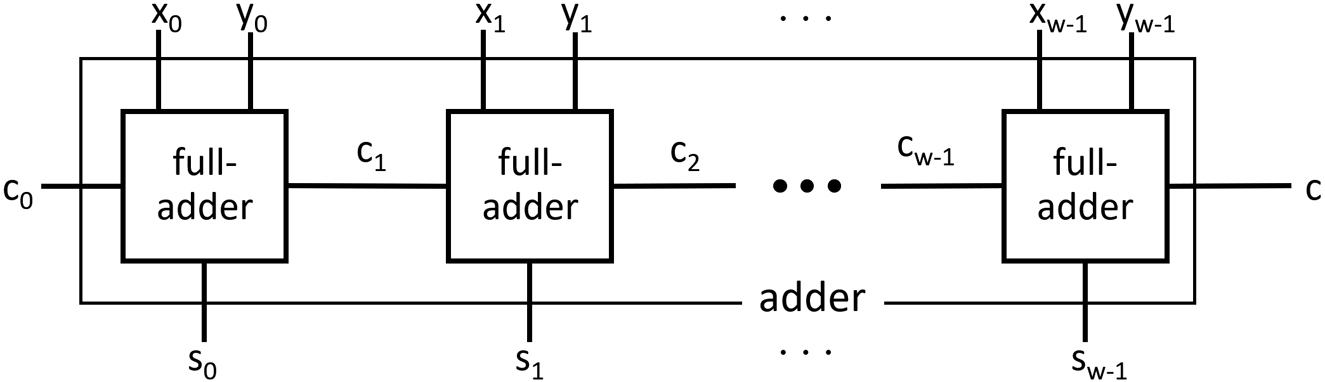
\includegraphics[scale=0.25]{Images/adder.png}
\todo{Improvised with PowerPoint. Redraw using Visio.}
\begin{Verbatim}
(defun adder (c0 x y)
  (if (consp x)
      (let* ((x0 (first x)) (xs (rest x))
             (y0 (first y)) (ys (rest y))
             (a0 (full-adder c0 x0 y0))
             (s0 (first a0)) (c1 (second a0)) ; {add.bit0}
             (a  (adder c1 xs ys))
             (ss (first a)) (c (second a)))
        (list (cons s0 ss) c))                ; {add1}
      (list nil c0)))                         ; {add0}
\end{Verbatim}
\end{center}
\caption{Ripple-Carry Adder and ACL2 Model}
\label{fig:adder}
\end{figure}

The ACL2 model in the figure relies
on inductive definition. It feeds the carry-in and
the low-order bits from the two numerals into a full adder.
(The low-order bit in a numeral is the ``ones bit,''
which is the first element of the list that we use to
represent the numeral.)
The sum bit from that full adder
is the low-order bit of the numeral representing the sum of
the numbers that the input numerals represent.
The remaining bits in that sum are those delivered by
the adder operating on the other bits in the input numerals
(that is, all the bits in the input numerals except the low-order bits).

Because the model defines an operator in ACL2,
you can run the operator to see that it works in specific cases.
To add two binary numerals, supply lists of 0s and 1s
representing those numerals in an invocation
of the adder operator, and specify zero as the input carry-bit.
The output will be binary numeral for the sum.

The theorem in Figure \ref{fig:adder-thm} (page \pageref{fig:adder-thm})
explains the details.
As with the two-bit adder (Figure \ref{adder2-ok}, page \pageref{adder2-ok})
the three numbers represented by the two input
numerals and the input carry, when added together,
equal the number represented
by a numeral formed from the output sum-bits and
the output carry-bit.
However, the theorem for the \emph{w}-bit adder
is stated as an implication to constrain
inputs to be numerals with the same number of bits.
This was not necessary with the theorem for the two-bit adder
because the lengths of the numerals were explicit in the ACL2 model.

\begin{figure}
\begin{center}
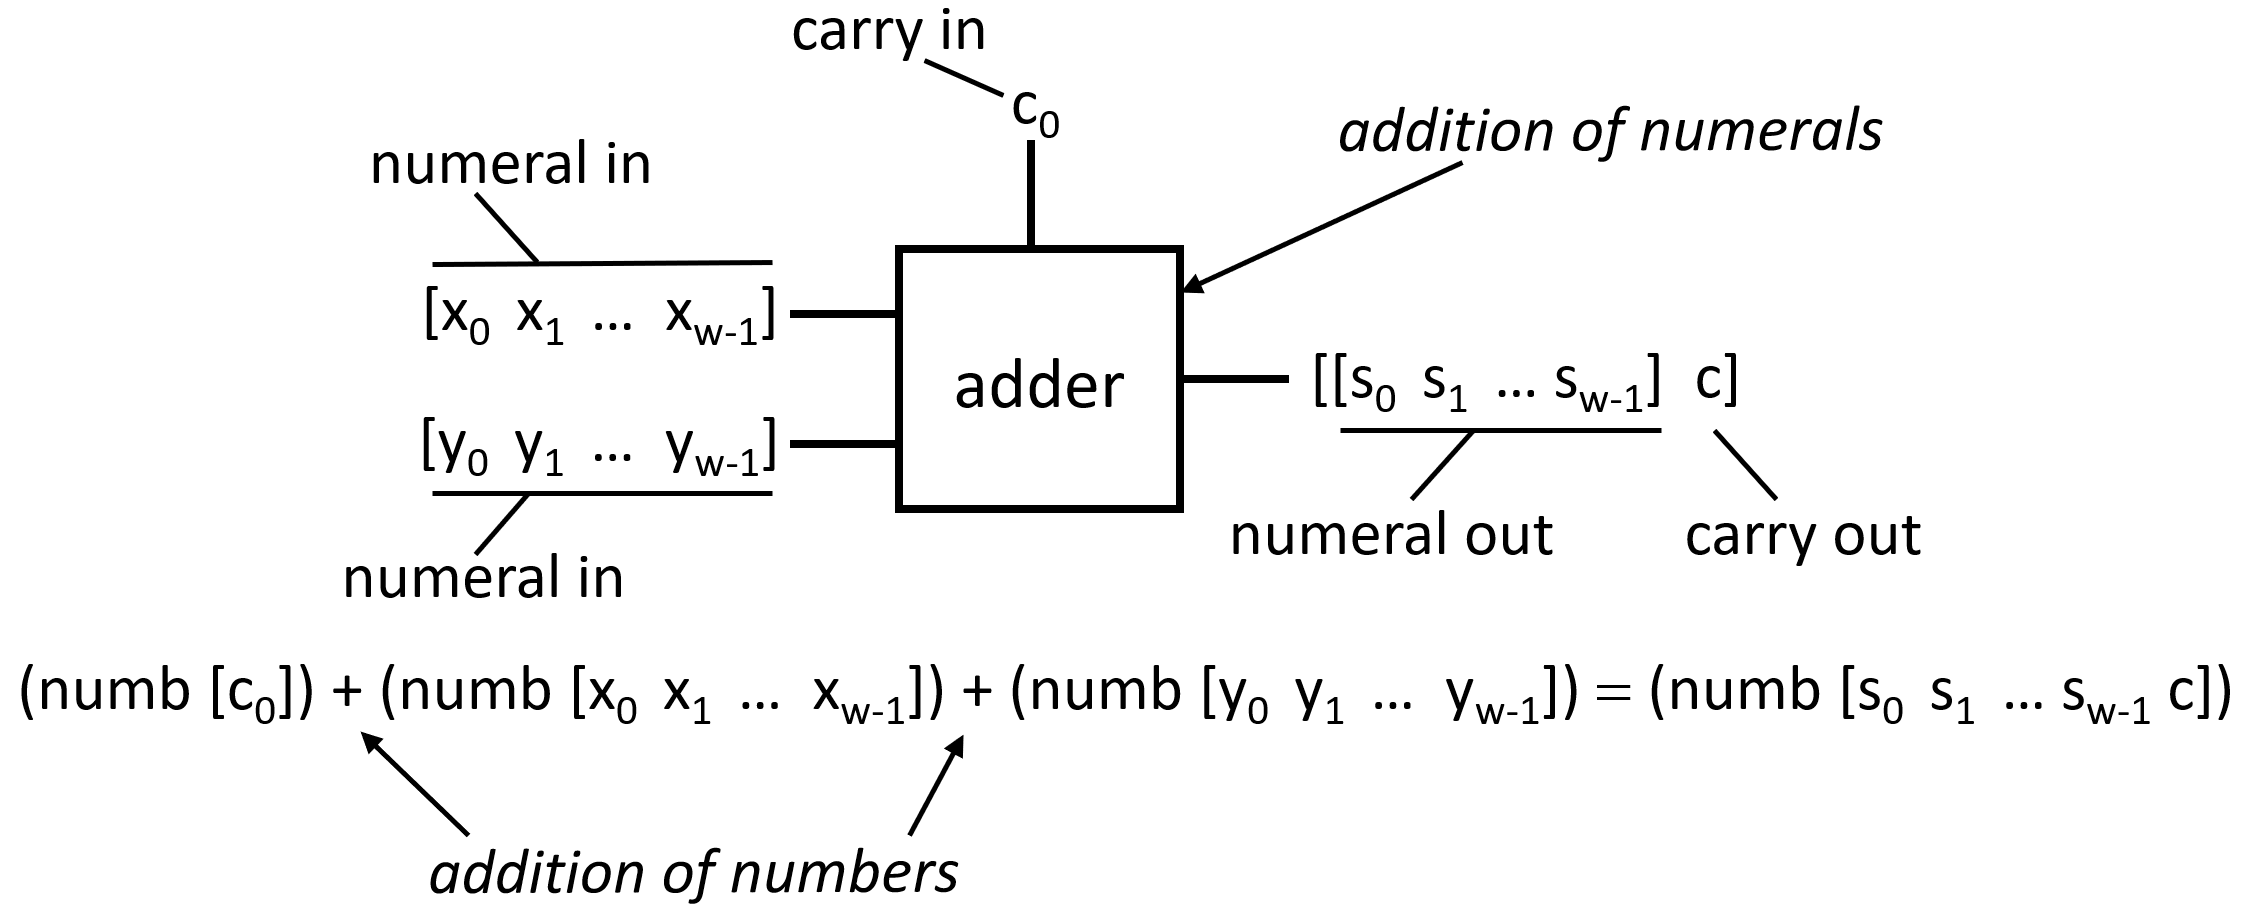
\includegraphics[scale=0.3]{Images/adder-thm.png}
\todo{Improvised with PowerPoint. Redraw using Visio.}
\begin{Verbatim}
(defthm adder-ok
  (implies (= (len x) (len y))
           (let* ((a (adder c0 x y))
                  (s (first a)) (c (second a)))
             (= (numb (append s (list c)))
                (+ (numb (list c0)) (numb x) (numb y))))))
\end{Verbatim}
\end{center}
\caption{Adding \emph{w}-Bit Binary Numerals}
\label{fig:adder-thm}
\end{figure}

Theorem \{\emph{adder-ok}\} (page \pageref{fig:adder-thm})
states the arithmetic property that
we expect the adder circuit is designed to have.
The mechanized logic of ACL2 succeeds in verifying
this theorem without assistance,
but because reasoning about circuits is such an important idea,
we think it will be worthwhile to go through
a paper-and-pencil proof.
Our proof will, of course, work from
the model of the adder circuit
(Figure \ref{fig:adder}, page \pageref{fig:adder}),
not from the circuit diagram.
Aside \ref{circuit-vs-model} (page \pageref{circuit-vs-model})
discusses some of the ramifications of this approach.

\begin{aside}
We expect that you could, given a basket of
logic gates, wires, and enough time,
use the diagram of the adder circuit to
build one for any specified word size,
and we think you can convince yourself that the model
matches the diagram.
If it does, then properties of the model
that we verify guarantee that the circuits also have those properties.

In a complete formalization, we would
need a way to convert models into instructions
for fabricating the circuits.
Formalizing the conversion to instructions a machine could
follow to fabricate a circuit, given an ACL2 model,
can be done using the methods
we have employed to formalize other operations.
However, in this treatment of the subject
we have left that step to the imagination.
\caption{Models and Circuit Fabrication}
\label{circuit-vs-model}
\end{aside}

\begin{samepage}
\label{adder-thm}
\begin{center}
\begin{tabular}{l}
Theorem \{\emph{adder ok}\} \\
(numb [$s_0$ $s_1$ \dots $s_{n}$ $c$]) $=$
(numb [$c_0$]) + (numb [$x_0$ $x_1$ \dots $x_{n}$]) + (numb [$y_0$ $y_1$ \dots $y_{n}$]) \\
where [[$s_0$ $s_1$ \dots $s_{n}$] [$c$]] $=$ (adder $c_0$ [$x_0$ $x_1$ \dots $x_{n}$] [$y_0$ $y_1$ \dots $y_{n}$])\\
\end{tabular}
\end{center}
\end{samepage}

Proving Theorem \{\emph{adder ok}\} amounts to
verifying that $(\forall n.R(n))$ is true,
where the predicate $R$ is defined on the natural numbers,
its universe of discourse, as follows.
\begin{center}
\begin{tabular}{l}
$R(n) \equiv$ $($(numb [$s_0$ $s_1$ \dots $s_{n}$ $c$]) $=$
(numb [$c_0$]) + (numb [$x_0$ $x_1$ \dots $x_{n}$]) + (numb [$y_0$ $y_1$ \dots $y_{n}$])$)$ \\
~~~~~ where [[$s_0$ $s_1$ \dots $s_{n}$] $c$] $=$ (adder $c_0$ [$x_0$ $x_1$ \dots $x_{n}$] [$y_0$ $y_1$ \dots $y_{n}$])\\
\end{tabular}
\end{center}

The proof will use mathematical induction.
To prove the base case $R(0)$,
we start our reasoning from the right-hand side of the equation.
The first step is
to compute the value of (adder $c_0$ [$x_0$] [$y_0$])
by working through the definition of the adder operator
(Figure \ref{fig:full-adder-thm}, page \pageref{fig:full-adder-thm}).
With these operands, the IF operator selects the inductive invocation \{add1\}:
[(cons $s_0$ $ss$) $c$], where [$ss$ $c$] $=$ (adder $c$ (rest [$x_0$]) (rest [$y_0$])).
The second and third operands in the invocation
are empty lists because (rest [$x_0$]) $=$ (rest [$y_0$]) $=$ nil.
The first operand is $c$, where [$s_0$ $c$] $=$ (full-adder $c_0$ $x_0$ $y_0$).
The theorem \{full-adder ok\} says that
(numb (full-adder $c_0$ $x_0$ $y_0$)) $=$ (numb [$c_0$]) + (numb [$x_0$]) + (numb [$y_0$]).
Therefore, (numb [$s_0$ $c$]) $=$ (numb [$c_0$]) + (numb [$x_0$]) + (numb [$y_0$]).

Figure \ref{fig:adder-thm-prf} (page \pageref{fig:adder-thm-prf}) sketches
this line of reasoning,
and presents a similar proof for the inductive case: $(R(n) \rightarrow R(n+1))$.
When the proof arrives at the sum
(numb [$c_1$]) $+$ (numb [$x_1$ \dots $x_{n+1}$]) $+$ (numb [$y_1$ \dots $y_{n+1}$]),
it recognizes that the induction hypthesis, $R(n)$, applies because
the numerals [$x_1$ \dots $x_{n+1}$] and [$y_1$ \dots $y_{n+1}$] have $n+1$
elements, like the numerals in the equation $R(n)$.
The subscripts run from $1$ to $n+1$ instead of from $0$ to $n$,
but it's the number of bits that counts, not their subscripts.
The induction hypothesis implies that this sum equals
(numb [$s_1$ \dots $s_{n+1}$ $c$]), and
the \{\emph{nmb1}\} theorem (Exercise \ref{nmb1}, page \pageref{nmb1})
combines this formula with (numb [$s_0$]) to arrive at left-hand side
of the equation $R(n+1)$, having started from the right-hand side.
By mathematical induction, we conclude that
the \{adder ok\} theorem is true.

The proof is tedious, to say the least.
It requires working out the details of
numerous operator invocations
from symbolic representations of the operands.
Fortunately, ACL2 is on hand to work through the
muck and mire and arrive at the same conclusion.
That gives us confidence that our ripple-carry circuit
for adding binary numerals delivers the expected results.

\begin{figure}
Theorem \{adder ok\}\\
$\forall n.($(numb [$s_0$ $s_1$ \dots $s_{n}$ $c$]) $=$
(numb [$c_0$]) + (numb [$x_0$ $x_1$ \dots $x_{n}$]) + (numb [$y_0$ $y_1$ \dots $y_{n}$])$)$\\
\hphantom{numb}where [[$s_0$ $s_1$ \dots $s_{n}$] $c$] $=$ (adder $c_0$ [$x_0$ $x_1$ \dots $x_{n+1}$] [$y_0$ $y_1$ \dots $y_{n}$])\\
\emph{Base Case}
\begin{center}
\begin{tabular}{l}
\hline
$R(0) \equiv$  $($(numb [$s_0$ $c$]) $=$ (numb [$c_0$]) + (numb [$x_0$]) + (numb [$y_0$])$)$ \\
 ~~~~~~ where [[$s_0$] $c$] $=$ (adder $c_0$ [$x_0$] [$y_0$]) \\
\hline
\end{tabular}
\begin{tabular}{ll}
(adder $c_0$ [$x_0$] [$y_0$]) $=$ [(cons $s_0$ nil) $c$] $=$ [[$s_0$] $c$] & \{\emph{add1}\} (\{\emph{adder}\} \emph{Fig. \ref{fig:adder}, p.\pageref{fig:adder}}) \\
~~~~ where [$s_0$ $c$] $=$ (full-adder $c_0$ $x_0$ $y_0$)          & \emph{note:} (adder $c$ nil nil) = [nil $c$] \\
(numb [$s_0$ $c$]) = (numb (full-adder $c_0$ $x_0$ $y_0$)          &  \\
~~~~~~~~~~~ $=$ (numb [$c_0$]) + (numb [$x_0$]) + (numb [$y_0$]))  & \{\emph{full-adder ok}\} \emph{(Fig. \ref{fig:full-adder-thm}, p.\pageref{fig:full-adder-thm})}\\
\end{tabular}
\end{center}
\emph{Inductive Case}
\begin{center}
\begin{tabular}{l}
 \hline
$R(n+1)$ $\equiv$ $($(numb [$s_0$ $s_1$ \dots $s_{n+1}$ $c$]) $=$ \\
\hphantom{$R(n+1)$ $\equiv$ $($}(numb [$c_0$]) $+$ (numb [$x_0$ $x_1$ \dots $x_{n+1}$]) $+$ (numb [$y_0$ $y_1$ \dots $y_{n+1}$])$)$ \\
 ~~~~~~ where [[$s_0$ $s_1$ \dots $s_{n+1}$] $c$] $=$ (adder $c_0$ [$x_0$ $x_1$ \dots $x_{n+1}$] [$y_0$ $y_1$ \dots $y_{n+1}$]) \\
\hline
\end{tabular}
\begin{tabular}{ll}
(numb [$c_0$]) $+$ (numb [$x_0$ $x_1$ \dots $x_{n+1}$]) $+$ (numb [$y_0$ $y_1$ \dots $y_{n+1}$])          & \\
$=$ (numb [$c_0$]) $+$ (numb [$x_0$]) $+$ $2\times$(numb [$x_1$ \dots $x_{n+1}$])                         & \{\emph{nmb1}\} \emph{(p. \pageref{nmb1})} \\
\hphantom{$=$ (numb [$c_0$]) }$+$ (numb [$y_0$]) $+$ $2\times$(numb [$y_1$ \dots $y_{n+1}$])                  & \{\emph{nmb1}\} \\
$=$ (numb [$c_0$]) $+$ (numb [$x_0$]) + (numb [$y_0$]) $+$                                                & \\
 ~~~~~~ $2\times($(numb [$x_1$ \dots $x_{n+1}$]) $+$ (numb [$y_1$ \dots $y_{n+1}$])$)$                    & \{\emph{algebra}\} \\
$=$ (numb (full-adder $c_0$ $x_0$ $y_0$)) $+$                                                             & \{\emph{full-adder ok}\} \\
 ~~~~~~ $2\times($(numb [$x_1$ \dots $x_{n+1}$]) $+$ (numb [$y_1$ \dots $y_{n+1}$])$)$                    & \\
$=$ (numb [$s_0$ $c_1$]) + $2\times($(numb [$x_1$ \dots $x_{n+1}$]) $+$ (numb [$y_1$ \dots $y_{n+1}$])$)$ & \{\emph{add.bit0}\} \emph{(\{adder\}}) \\
$=$ (numb [$s_0$]) $+$ $2\times$(numb [$c_1$]) +                                                          & \{\emph{nmb1}\} \\
\hphantom{$=$ (numb [$s_0$ $c_1$]) + }$2\times($(numb [$x_1$ \dots $x_{n+1}$]) $+$ (numb [$y_1$ \dots $y_{n+1}$])$)$  & \\
$=$ (numb [$s_0$]) $+$                                                                                    & \{\emph{algebra}\} \\
 ~~~~~~ $2\times($(numb [$c_1$]) $+$ (numb [$x_1$ \dots $x_{n+1}$]) $+$ (numb [$y_1$ \dots $y_{n+1}$])$)$ & \\
$=$ (numb [$s_0$]) $+$ $2\times$(numb [$s_1$ \dots $s_{n+1}$ $c$])                                        & \{$R(n)$\} \\
$=$ (numb [$s_0$ $s_1$ \dots $s_{n+1}$ $c$])                                                              & \{\emph{nmb1}\} \\
\end{tabular}
\end{center}
\caption{Theorem \{adder ok\} and Proof by Mathematical Induction}
\label{fig:adder-thm-prf}
\end{figure}

\begin{aside}
A ``word'' in a computer is a collection of bits
that the computer treats as a whole in certain operations,
especially arithmetic operations.
A circuit to perform arithmetic will carry out
the operation on words denoting binary numerals.
Since all words have the same number of bits,
both of the numerals supplied as inputs to circuit
for an arithmetic operator will have the same number of bits.

We could change the design of the circuit for the adder
to accommodate input numerals of differing lengths.
However, since we are modeling a circuit
in which the input numerals have the same length,
the model does not need to account for that possibility.
\caption{Adder Circuit and Numerals of Different Lengths}
\label{adder-circuit-and-numerals-of-different-lengths}
\end{aside}

\begin{ExerciseList}
\Exercise \label{ex:add-bin}
Define in ACL2 a operator ``add-bin''
that adds any two binary numerals,
even if the numerals contain a different number of bits.
That is, the value (add-bin $c$ $x$ $y$) should be a binary numeral
for the number (numb [$c$] + (numb $x$) + (numb $y$)),
as long as $x$ and $y$ are binary numerals and $c$ is 0 or 1,
regardless of (len $x$) or (len $y$).
Design and run some sanity checks on your operator.

\Exercise Define in ACL2 a theorem about the operator add-bin (Excercise \ref{ex:add-bin})
that is analogous to theorem \{adder ok\}
(Figure \ref{fig:adder-thm-prf}, page \pageref{fig:adder-thm-prf}).

\end{ExerciseList}

\section{Numerals for Negative Numbers}
\label{sec:negative-numerals}

So far, all the numerals we've seen have denoted positive numbers.
An arithmetic device also needs to deal with negative numbers,
and there are many ways to do that.
The most common method is known as the
``twos-complement'' system.

Twos-complement numerals are a special interpretation of
ordinary binary numerals.
For numbers in the range $0$, $1$, $\dots$ $(2^{w-1}-1)$,
where \emph{w} is the ``word size''
of the circuits for arithmetic operations,
twos-complement numerals are ordinary binary numerals.
All of the numerals for this set of numbers
have $(w-1)$ or fewer bits,
not counting leading zeros
(Theorem \{\emph{len-bits}$\le$\}, page \pageref{len-bitsLE}).
To make the numerals match the word size,
the twos-complement system pads them with leading zeros
to make them have exactly \emph{w} bits.
Leading zeros don't change the number that a numeral denotes
(Theorem \{\emph{leading-0s}\}, page \pageref{leading-0s}), but,
as with the ripple-carry adder (Figure \ref{fig:adder}, page \pageref{fig:adder}),
circuits to perform arithmetic on twos-complement numbers will
require exactly \emph{w} bits for each input numeral
because there are $w$ input lines for each addend,
and each input line must carry a signal
for either a zero-bit or a one-bit.
So, the non-negative numbers, $0$, $1$, \dots $(2^{w-1}-1)$
consume half of the $2^w$ bit-patterns available with
\emph{w}-bit words.

For negative numbers,
the twos-complement system uses the other half of the bit-patterns.
These are the numerals that would normally denote numbers in the range
$2^{w-1}$, $(2^{w-1}+1)$, \dots $(2^{w}-1)$.
If $(-n)$ is a negative number in the range $-2^{w-1} \leq (-n) < 0$,
\label{2s-def}
then the twos-complement numeral for $(-n)$
is the ordinary binary numeral for $(2^w - n)$.
Since $2^{w-1} = (2^{w}-2^{w-1}) \leq (2^w - n) < 2^w$,
this numeral has exactly \emph{w} bits
(Theorem \{\emph{len-bits}\}, page \pageref{len-bits}).
We also know that its high-order bit is a one-bit
(Theorem \{\emph{hi-1}\}, page \pageref{hi-1}),
so there is an easy way to recognize numerals that denote negative numbers.

For example, a computer with 32-bit words that uses
two-complement numerals has arithmetic circuits that
deal with numbers $n$ in the range $-2^{w-1} \leq n < 2^{w-1}$.
In the positive part of the range, it represents numbers as
ordinary binary numerals, but with enough leading zeros
to fill the 32-bit word.
For a number ($-n$) in the negative part of the range,
the twos-complement system uses the binary numeral
for ($2^{32}-n$) to represent the number ($-n$).
Since ($-n$) is in the range
$-2^{31} \le -n < 0$, we can assert that
$2^{31} \le 2^{32}-n < 2^{32}$.
Therefore, the twos-complement, binary numeral
for the negative number ($-n$)
has exactly 32 bits (Theorem \{\emph{len-bits}\}, page \pageref{len-bits}).

Modular arithmetic makes twos-complement numerals
for negative numbers act like the negative numbers they stand for
when they are added to other numerals.
For negative numbers ($-n$) in the range $-2^{31} \le -n < 0$,
the value of (($-n$) mod $2^{32}$) is ($2^{32}-n$).
Therefore, since addition and subtraction
in modular arithmetic is consistent with ordinary addition and subtraction
(page \pageref{modular-arithmetic}), it follows that
  ($(m+(-n))$ mod $2^{32}$
= (($m$ mod $2^{32}$) + ($(-n)$ mod $2^{32}$)) mod $2^{32}$
= (($m$ mod $2^{32}$) + ($(2^{32} - n)$ mod $2^{32}$)) mod $2^{32}$.

That is, adding the numbers represented by twos-complement
numerals, including numbers in the negative range,
is just like adding ordinary numbers in modular arithmetic.
Subtraction is handled by negating a number
(that is, computing the twos-complement representation
of its negative), then performing addition modulo $2^{32}$.

The same thing works for any word size.
With word size $w$, the twos complement system
handles addition and subtraction for numbers
in the range $-2^{w-1}, \dots -1, 0, 1, 2, \dots 2^{w-1}-1$
by performing ordinary addition of numerals,
as with the ripple-carry adder, but interpreting
the numerals according to the twos-complement scheme.
Circuits for performing addition (and subtraction, since
it is the same operation in a twos-complement system)
take advantage of the consistency between modular arithmetic
and ordinary arithmetic (page \pageref{modular-arithmetic}).

In summary, the twos-complement representation for computers with
word size $w$ deals with numbers $n$ in the range
$-2^{w-1} \leq n < 2^{w-1}$.
We will refer to this set of integers as $I(w)$.
\label{def-Iw}
\begin{center}
$I(w) = \{-2^{w-1}, \dots -1, 0, 1, 2, \dots 2^{w-1}-1\}$
\end{center}

Twos-complement numerals for numbers in the negative range
have exactly $w$ bits, with a one-bit in the high-order slot.
Twos-complement numerals for numbers in the positive range of $I(w)$
take the form of ordinary binary numerals, except that
they are padded with enough leading zeros
to fill out a $w$-bit word, where $w$ is the word size of the computer.
The ``twos'' operator, defined as follows, delivers the twos-complement numeral
for a number $n$ in the set $I(w)$.

\label{twos-defun}
\begin{Verbatim}
(defun twos (w n)             ; w = word size
  (if (< n 0)                 ; -2^(w-1) <= n < 2^(w-1)
      (bits (+ (expt 2 w) n)) ; {2s-}
      (pad w 0 (bits n))))    ; {2s+}
\end{Verbatim}

The twos operator uses the operator bits (page \pageref{bits-defun})
to compute binary numerals.
For negative numbers it adds $2^w$
(that is, (expt $2$ $w$), referring to the ACL2 intrinsic operator expt)
before computing the numeral.
For non-negative numbers, it computes the numeral,
then uses the pad operator (page \pageref{pad-defun})
to insert leading zeros to match the word-size.
There will always be some padding for numerals representing
numbers in the positive range because
$0 \le n < 2^{w-1}$ implies that
$0 \le $(len (bits $n$)) $< w$
(Theorem \{\emph{len-bits}$\le$\}, page \pageref{len-bitsLE}).

Figure Figure~\ref{fig:2s-comp-3bit} displays
twos-complement numerals for the numbers in the set $I(3)$.
Of course, this example is just to illustrate the idea.
Three is a ridiculously small word size.
No computer would have three-bit words,
but the example gets the point across with a table of manageable size.

\begin{figure}
\begin{center}
\begin{tabular}{cccc}
 $n \in I(3)$ & $2^3+n$  & (twos $3$ $n$)   & \emph{binary numeral} \\
 $-4$         & $4$      & [0 0 1]          & 100                   \\
 $-3$         & $5$      & [1 0 1]          & 101                   \\
 $-2$         & $6$      & [0 1 1]          & 110                   \\
 $-1$         & $7$      & [1 1 1]          & 111                   \\
 $~~0$        &          & [0 0 0]          & 000                   \\
 $~~1$        &          & [1 0 0]          & 001                   \\
 $~~2$        &          & [0 1 0]          & 010                   \\
 $~~3$        &          & [1 1 0]          & 011                   \\
\end{tabular}
\\ $I(w) = I(3) = \{-2^{3-1}=-4, -3, -2, -1, 0, 1, 2, 3=2^{3-1}-1\}$
\\ \emph{word size} $w = 3$
\end{center}
\caption{Twos-Complement Numerals for 3-bit Words}
\label{fig:2s-comp-3bit}
\end{figure}

If the input carry is zero and
the input numerals are interpreted
as twos-complement numerals for numbers in the set $I(w)$,
then the sum-bits of the output numeral from the ripple-carry adder
(Figure \ref{fig:adder}, page \pageref{fig:adder})
form the twos-complement numeral for the sum of the input numerals.
The carry output from the circuit can be used to determine
whether or not the sum is in the set $I(w)$ of numbers representable
by \emph{w}-bit, twos-complement numerals.\footnote{The
output carry can be used to perform multi-word arithmetic
or to detect overflow conditions. Adding two numbers, $m+n$,
that are both in the top half of the positive range
($2^{w-2} \leq m, n < 2^{w-1}$) produces a number that is
outside the set $I(w)$, so the sum has no \emph{w}-bit, twos-complement numeral.
This outcome is known as an overflow.
Similarly, adding two numbers in the bottom half of the
negative range ($-2^{w-1} \leq m,n < -2^{w-2}$)
produces a number outside the twos-complement range, an overflow.}

Now, here is an interesting trick
for computing the twos-complement numeral of a negative number without
computing $2^w$ or doing subtraction.
It works like this.
Let $x_{w-1}x_{w-2} \dots x_2x_1x_0$
be the $w$-bit, binary numeral for a number $n$ in the range $1$, $2$, \dots $2^{w-1}$,
padded if necessary with leading zeros to fill out the full $w$ bits.
Then, the twos-complement numeral for $(-n)$ can be computed
in a two-step procedure.
First, invert the bits: change the zero-bits to one-bits,
and change the one-bits to zero-bits.
Then, use the ripple-carry adder to add the numeral for the number $1$
to the numeral with the inverted bits.
The result will be the twos-complement numeral for $(-n)$.
The same trick works to negate the twos-complement numeral
of a number $(-n)$ from the range $-2^{w-1} < -n \leq 0$.

The trick does not work for the number $-2^{w-1}$
because the negative of that number (namely, $2^{w-1}$)
is outside of the set $I(w)$,
so it doesn't have a \emph{w}-bit, twos-complement numeral.
The trick does work for negating the twos-complement numeral for zero.
In that case the procedure delivers an output numeral identical
to the input (namely, a numeral consisting of \emph{w} zero-bits).
It produces a one-bit for the carry-out, but that bit is not part of the numeral.
Figure~\ref{fig:2s-comp-negation}
(page \pageref{fig:2s-comp-negation})
explains how inverting the bits and adding one leads to the negation
of the input numeral.
It's an exercise in algebra and modular arithmetic.\footnote{The
proof of the \{$ys$ increment\} equation
in Figure~\ref{fig:2s-comp-negation}
cites a formula for the sum of a geometric progression.
The formula is proved at, for example, \url{https://en.wikipedia.org/wiki/Geometric_progression}.}

\begin{figure}
\emph{Some facts, notation, and equations:}
\begin{center}
\begin{tabular} {ll}
$1 \le n \le 2^{31}$                                   & \emph{range of numbers to negate} \\
(len (bits $n$)) $\le w$                               & \{\emph{len-bits}$\le$\} \emph{(page \pageref{len-bitsLE})} \\
$xs$ = {[$x_0$ $x_1$ \dots  $x_{w-1}$]}                & $xs$ = (pad $w$ 0 (bits $n$))\emph{, padded binary numeral} \\
(numb $xs$) = $n$                                      & \{\emph{leading-0s}\} \emph{(page \pageref{leading-0s})} \\
$ys$ = [$y_0$ $y_1$ \dots $y_{w-1}$]                   & \emph{inverted bits} $y_i = 1 - x_i$ \emph{(0s for 1s, 1s for 0s)} \\
$1$ $+$ (numb $ys$) $=$ $2^w - n$                      & \{$ys$ \emph{increment}\} \emph{equation (see proof below)} \\
(bits (+ 1 (numb $ys$))) $=$ (twos $w$ $(- n)$)        & \{\emph{2s trick}\} \emph{equation (see proof below)} \\
\end{tabular}
\end{center}
\emph{Proof of} \{$ys$ \emph{increment}\} \emph{equation:} $1$ $+$ (numb $ys$) $=$ $2^w - n$
\begin{center}
\begin{tabular} {lllll}
  & $1$   &$+ $ &(numb $ys$)                                                   &  \\
= & $1$   &$+ $ &$y_02^0 + y_12^1 + \dots + y_{w-1}2^{w-1}$                    & \{\emph{Horner 2}\}  \\
= & $1$   &$+ $ &$(1 - x_0)2^0 + (1 - x_1)2^1 + \dots ++ (1 - x_{w-1})2^{w-1}$ & $\forall i.(y_i = 1-x_i)$ \\
= & $1$   &$+ $ &$(2^0 + 2^1 + \dots + 2^{w-1})$                               & \{\emph{algebra}\}   \\
  &       &$- $ &$(x_02^0 + x_12^1 + \dots + x_{w-1}2^{w-1})$                  &                      \\
= & $1$   &$+ $ &$(2^w - 1) - (x_02^0 + x_12^1 + \dots + x_{w-1}2^{w-1})$      & \{\emph{geometric progression}\} \\
= & $2^w$ &$- $ &$(x_02^0 + x_12^1 + \dots x_{w-1}2^{w-1})$                    & \{\emph{algebra}\} \\
= & $2^w$ &$- $ &(numb $xs$)                                                   & \{\emph{Horner 2}\}   \\
= & $2^w$ &$- $ &$n$                                                           & (numb $xs$) = $n$     \\
\end{tabular}
\end{center}
\emph{Proof of} \{\emph{2s trick}\} \emph{equation:} (bits (+ 1 (numb $ys$))) $=$ (twos $w$ $(- n)$)
\begin{center}
\begin{tabular} {lll}
  & (bits (+ 1 (numb $ys$)))        & \\
= & (bits $(2^w - n)$)              & \{$ys$ \emph{increment}\} \emph{equation} \\
= & (bits $(2^w + (- n))$)          & \{\emph{algebra}\}                        \\
= & (bits (+ (expt 2 $w$) $(- n)$)) & $(2^w + (- n))$ \emph{in ACL2 notation}   \\
= & (twos $w$ $(- n)$)              & \{$2s-$\} \emph{(}\{\emph{twos}\}\emph{, page \pageref{twos-defun})} \\
\end{tabular}
\end{center}
\caption{Twos-Complement Negation Trick}
\label{fig:2s-comp-negation}
\end{figure}

\begin{ExerciseList}

\Exercise \label{len-2s}
Prove \{\emph{len-2s}\}:
$\forall w$.($(n \in I(w)) \rightarrow$ ((len (twos $w$ $n$)) $= w$))

\Exercise \label{minus-sign}
Prove \{\emph{minus-sign}\}:
$\forall n \in I(w).((n < 0) \rightarrow$ (fin(twos $w$ $n$)) = 1) \\
The operator fin is defined on page \pageref{fin-defun}.

\Exercise \label{plus-sign} Prove \{\emph{plus-sign}\}:
$\forall n \in I(w).((n \ge 0) \rightarrow$ (fin(twos $w$ $n$)) = $0$)

\Exercise \label{2s-negation-circuit}
Diagram a negation circuit that transforms its input,
which is the twos-complement numeral for a number $n$ in the range
$-2^{w-1} < n < 2^{w-1}$,
into the twos-complement numeral for $(-n)$ as output.
In your diagram, rely on the twos-complement negation trick
(Figure~\ref{fig:2s-comp-negation},
and use the gate-like symbol in
Figure \ref{fig:adder-thm} (page \pageref{fig:adder-thm})
to depict the ripple-carry adder circuit.
(\emph{Note}: Your circuit will also produce the twos-complement
numeral for $-2^{w-1}$, given the binary numeral for $2^{w-1}$
as input.)

\Exercise \label{2s-negation-circuit-model}
Define an ACL2 model for the negation circuit
of Exercise~\ref{2s-negation-circuit}.
Your model may refer to the ACL2 model
of the ripple carry adder in
Figure \ref{fig:adder} (page \pageref{fig:adder}).

\Exercise Define and run a doublecheck property that
tests the correctness of
an ACL2 model of the negation circuit of
Excercise~\ref{2s-negation-circuit-model}.

\Exercise \label{2s-subtraction-circuit}
Diagram a circuit that subtracts twos-complement numerals.
In your diagram, use the gate-like symbol in
Figure \ref{fig:adder-thm} (page \pageref{fig:adder-thm})
to depict the ripple-carry adder circuit,
and use a similar, gate-like symbol for the negation circuit
of Exercise~\ref{2s-negation-circuit}.

\Exercise \label{2s-subtraction-circuit-model}
Define an ACL2 model of the twos-complement
subtraction circuit of Exercise~\ref{2s-subtraction-circuit}.

\Exercise Define and run a doublecheck property that
tests the correctness of
the ACL2 model of the subtraction circuit
in Exercise~\ref{2s-subtraction-circuit-model}.

\Exercise \label{2s-comparison-circuit}
Diagram a comparison circuit that takes a pair of
twos-complement numerals as inputs and delivers a one-bit
if the first number is greater than the second
and a zero-bit otherwise.
In your diagram, use a gate-like symbol
for the subtraction circuit of Exercise~\ref{2s-subtraction-circuit}.
\emph{Hint}: Apply theorems \{\emph{minus-sign}\} and \{\emph{plus-sign}\}
from Exercises~\ref{minus-sign} and \ref{plus-sign}.

\Exercise \label{2s-comparison-circuit-model}
Define an ACL2 model of the comparison circuit
of Exercise~\ref{2s-comparison-circuit}.
Your model may refer to the subtraction circuit model
of Exercise~\ref{2s-subtraction-circuit-model}.

\Exercise Define and run a doublecheck property
that tests the correctness of the comparison circuit model
of Exercise~\ref{2s-comparison-circuit-model}.

\end{ExerciseList}

%%% Local Variables:
%%% mode: latex
%%% TeX-master: "book"
%%% End:
